\documentclass[11pt]{article}
\usepackage[parfill]{parskip}
\usepackage{graphicx}
\usepackage{wrapfig}
\usepackage{subcaption}
\usepackage[top=1in, bottom=1in, left=1in, right=1in]{geometry}
\bibliographystyle{plain}
\usepackage{amsmath}
\usepackage{amsfonts}
\usepackage{hyperref}
%%%%%%%%%%%%%%%%%%%%%%%%%%%%%%%%%%%%%%%%%%%%%%%%%%%%%%%%%%%%%%%
\usepackage{fancyhdr}
\pagestyle{fancy}
%%% Please add the author's last names
\lhead{Galois TA2 AMIDOL}
\rhead{ASKE Milestone 2}
%%% Please use \cfoot{} to remove page numbers
\cfoot{ }
\renewcommand{\headrulewidth}{0pt}
\renewcommand{\footrulewidth}{0pt}
%%%%%%%%%%%%%%%%%%%%%%%%%%%%%%%%%%%%%%%%%%%%%%%%%%%%%%%%%%%%%%&
\usepackage{titlesec}
\titlespacing{\section}{0pt}{\parskip}{-.5\parskip}
\titlespacing{\subsection}{0pt}{\parskip}{- .5\parskip}
\titlespacing{\subsubsection}{0pt}{\parskip}{- .5\parskip}
\newcommand{\closeup}{\setlength{\itemsep}{-4pt}}

\newcommand{\amidol}{\textsc{AMIDOL}}

\def\signed #1{{\leavevmode\unskip\nobreak\hfil\penalty50\hskip2em
  \hbox{}\nobreak\hfil(#1)%
  \parfillskip=0pt \finalhyphendemerits=0 \endgraf}}

\newsavebox\mybox
\newenvironment{aquote}[1]
  {\savebox\mybox{#1}\begin{quote}}
  {\signed{\usebox\mybox}\end{quote}}

\date{\vspace{-5ex}}
% Use this to get rid of the date

\usepackage{authblk}
\author[1]{Eric Davis}
\author[1]{Alec Theriault}
\author[1]{Max Orhai}
%\author[1]{Eddy Westbrook}
\author[1]{Ryan Wright}
\affil[1]{Galois, Inc}

%\setcounter{page}{0}



\title{ASKE Milestone 2 for \amidol{}}

\begin{document}
\maketitle
\vspace{10pt}

\section{Introduction}

Complex system analysis currently requires teams of domain experts, data scientists, mathematicians, and software engineers to support the entire life cycle of model-based inference.  The models that result are often bespoke, lack generalizability, are not performable, and make it difficult to synthesize actionable knowledge and policies from their raw outputs.  In this report we describe the current prototype system for \amidol{}: the Agile Metamodel Interface using Domain-specific Ontological Languages, a project that aims to reduce the overhead associated with the model life cycle and enables domain experts and scientists to more easily build, maintain, and reason over models in robust and highly performable ways, and to respond rapidly to emerging crises in an agile and impactful way.  We discuss the current design principles of the \amidol{} prototype, its capabilities, plans for development, and formal aspects of the system.

\amidol{} is designed to support models in a number of scientific, physical, social, and hybrid domains by allowing domain experts to construct meta-models in a novel way, using visual domain specific ontological languages (VDSOLs).  These VDSOLs utilize an underlying intermediate abstract representation to give formal meaning to the intuitive process diagrams scientists and domain experts normally create.  \amidol{}'s abstract representations are executable, allowing \amidol{}'s inference engine to execute prognostic queries on reward models and communicate results to domain experts. \amidol{} binds results to the original ontologies providing more explainability when compared to conventional methods.

\amidol{} addresses the problem of machine-assisted inference with two high-level goals:

\begin{enumerate}
\item improving the ability of domain experts to build and maintain models and
\item improving the explainability and agility of the results of machine-inference.
\end{enumerate}

Our techniques for achieving these goals incorporate abstract functional representations, intermediate languages, and semantic knowledge representation and binding in graph structures into traditional machine learning and model solution techniques.

\section{VDSOL Definition}

\amidol{} is designed to support the definition of ontological languages which describe systems as formal objects.  Objects for a given domain are organized into \emph{toolkits} consisting of \textbf{nouns} and \textbf{verbs}.  Nouns define elements which make up the state space of a system, and verbs define transitions in the state space.  VDSOLs enable domain experts to build models of complex systems which are easier to maintain, validate, and verify, and avoid common pitfalls of monolithic and hand-coded implementations.  To provide visual context for modelers, \amidol{} supports the use of arbitrary scalable vector graphics (SVGs) to represent nouns and verbs, and features a canvas to draw nouns and verbs with labeled arcs connecting them to provide context.

The goal of \amidol{}'s VDSOLs is to enable domain experts to define their models using an interface and visual language similar to the semi-formal diagrams they use today, but with the advantage that \amidol{}s VDSOLs have formal, executable, meaning.  VDSOLs provide a performable, reusable, system for scientists to use when attempting to derive insights relating to the complex systems they represent.

VDSOLs in \amidol{} are constructed using a graphical user interface implemented using asynchronous javascript and XML to build a responsive interface to define models of complex systems, reward models used to explore and understand complex system behavior, and to interact with the results of solvers implemented in the Machine-Assisted Inference Engine.

\subsection{Basic Language Properties}
\paragraph{Nouns}: Nouns in \amidol{} represent portions of the model associated with its state space.  The \amidol{} IR translates noun elements into state variables and constants.  Nouns are represented by custom SVGs, and can be connected to verbs which act upon them.  Users can set the label associated with a noun, which impacts the naming of state variables associated with the noun.

\paragraph{Verbs}: Verbs in \amidol{} represent activities or events which can occur in a model, and which act upon nouns changing the state of the system.  Verbs are associated with a few mandatory and optional properties which impact their translation into the intermediate representation.  All verbs have a mandatory rate which defines the rate at which the associated event occurs.  This rate can be dependent on nouns in the model.  Verbs have an optional enabling condition which can be dependent on nouns in the model.  The enabling condition defines that state variable bounds during which the associated event is enabled, and can be specified as an algebraic expression over state variables associated with nouns in a model.  Verbs also have an optional output function which defines which nouns are impacted when the associated event fires.

\subsection{Composability of Atomic Models}

\amidol{} is being designed to support the composition of individual models to enable model reuse, compositional methods for solution, to enhance backend support for performance optimizations that require symmetry detection, and to allow domain scientists to experiment by swapping out components of a model which may represent complex hypotheses about individual elements.  Model composition in \amidol{} is being designed to support two primary mechanisms: \emph{state-sharing} \cite{sanders1992dependability,sanders1988construction} and \emph{event-synchronization} \cite{lampka2002symbolic}.

State-sharing allows model composition by defining an interface for a model in the form of a set of state variables, which are then "shared" with another model.  Shared state-variables in two composed models have the same marking, or value, and are effected by events in both models.  Event-synchronization functions in an analogous way, allowing two events to be paired, such that the input predicate and output predicate of the new shared event is the union of the predicates of the events being shared.

\amidol{} is planned to support both replicate and join operations defined over Petri-nets and stochastic activity networks. \cite{sanders1995ultrasan}  In addition to replicate and join operations, \amidol{} will support a novel model composition relation allowing users to specify sub-models as nouns and verbs which can be connected to existing components using Abstract Base Models, based on class inheritance patterns \cite{bruce2002foundations}, which allows users to specify abstract models with undefined states and events.

\section{Abstract Intermediate Representation}

The Abstract Intermediate Representation (IR) for \amidol{} is meant to be a universal way to specify models, regardless of their domain, and provides a Turing-complete way to specify models performably, while avoiding domain specific considerations.

The intermediate representation employed by \amidol{} has its roots in Markov models \cite{howard2012dynamic}, Generalized Stochastic Petri-nets with inhibitor arcs \cite{chiola1993generalized} which have been shown to be Turing complete, and stochastic activity networks \cite{movaghar1985performability,sanders2000stochastic} which are extensions of Petri-nets that allow more compact model specification.  \amidol{} currently extends these concepts primarily by creating ways to link to the original ontology of nouns and verbs, and by allowing embedded reward structures to be linked to a graph-based results database which stores the outcomes of experiments and can be used for the construction of arbitrary measures on the underlying model to support inference needs.

\subsection{Language Properties}

Formally, the IR is a 5-tuple, $(S, E, L, \Phi, \Lambda, \Delta)$ where:
\begin{itemize}
\item $S$ is a finite set of state variables $\{s_0, s_1, \ldots, s_{n-1}\}$ that take on values in $\mathbb{N}$.
\item $E$ is a finite set of events $\{e_0, e_1, \ldots, e_{m-1}\}$ that may occur in the model.
\item $L: S|E \rightarrow \mathbb{N}$ is the event and state variable labeling function that maps elements of $S and E$ into the original ontology.
\item $\Phi: E \times N_0 \times N_1 \times \ldots \times N_{n-1} \rightarrow \{0, 1\}$ is the event enabling predicate.
\item $\Lambda: E \times N_0 \times N_1 \times \ldots \times N_{n-1} \rightarrow (0, \infty)$ is the transition rate specification.
\item $\Delta: E \times N_0 \times N_1 \times \ldots \times N_{n-1} \rightarrow N_0 \times N_1 \times \ldots \times N_{n-1}$ is the state variable transition function specification.
\end{itemize}

Informally the IR represents models defined in a given VDSOL using an formalism based on Generalized Stochastic Petri-nets with inhibitor arcs (which have the result of making Petri-nets Turing complete).  Instead of inhibitor arcs, we utilize the more intuitive and performable method of allowing events to have input predicates ($Phi$) which can be evaluated to determine if an event is enabled, and output predicates which define the side effects of event firing.

\paragraph{State variables}: intuitively, state-variables make up the current state of the model, and measure the configuration and capabilities of all modeled components.  While state variables are defined as taking on values in $\mathbb{N}$, this does not restrict them from representing real numbers to arbitrary precision in modern computer hardware.  In practice, they are implemented as integers, and floating point numbers by the \amidol{} source code.

\paragraph{Events}: events, when fired, change the state of a model by altering the value of state variables.  Events in \amidol{} are associated with input predicates, output predicates, and a rate function which returns the next firing time of a given event.  The rate function is an expression over random variable distributions.

\paragraph{Input predicates}: an input predicate is associated with an event, and a potentially empty set of state variables.  Input predicates are functions of the marking of their set of variables which map the markings of those variables onto the set $\{1, 0\}$.  For those markings in which the input predicate evaluates to $1$, the event is considered enabled and will fire as normal.  For those markings in which the input predicate evaluates to $0$, the event is considered disabled and cannot fire until subsequently enabled.

\paragraph{Output predicates}: an output predicate is associated with an event, and a potentially empty set of state variables.  Output predicates map a set of state variables, and their marking, to a new marking for the same state variables and define the side effects of event firing on the state of the model.

\section{Reward Variables, Reward Models, and Inference}

The \amidol{} intermediate representation allows for the specification of reward variables or structures over a given model, and the composition of these structures with a model to produce composed models which can then be solved by the inference engine.  Given a model $M = (S, E, L, \Phi, \Lambda, \Delta)$ we define two basic types of rewards structures, rewards over state variable values (rate rewards), and rewards over events (impulse rewards).

\cite{qureshi1996algorithms,deavours1999efficient,ciardo1996well,sanders1991reduced}

\subsection{Rate Reward Variables}

A rate reward is formally defined as a function $\mathcal{R}: P(S, \mathbb{N}) \rightarrow \mathbb{R}$ where $q \in P(S, \mathbb{N})$ is the reward accumulated when for each $(s,n) \in q$ the marking of the state variable $s$ is $n$.  Informally a rate reward variable $x$ accumulates a defined reward whenever a subset of the state variables take on prescribed values.

\subsection{Impulse Reward Variables}

An impulse reward is formally defined as a function $\mathcal{I}: E \rightarrow \mathbb{R}$ where $e \in E, \mathcal(I)_e$ is the reward for the completion of $e$.  Informally an impulse reward variable $x$ accumulates a defined reward whenever the event $e$ fires.

\subsection{Temporal Characteristics of Reward Variables}

Both rate and impulse reward variables measure the behavior of a model $M$ with respect to time.  As such, a reward variable $\theta$ is declared as either an instant-of-time variable, an interval-of-time variable, a time-averaged interval-of-time variable, or a steady state variable.  An instant of time variable $\Theta_t$ is defined as:

\[ \theta_t = \sum_{\nu \in P(S, \mathbb{N})} \mathcal{R}(\nu) \cdot \mathcal{I}^{\nu}_t + \sum_{e \in E} \mathcal{I}(e) \cdot I_t^e\]

Intuitively a rate reward declared as an instant-of-time variable \cite{freire1990technique} can be used to measure the value of a state variable precisely at time $t$, and an impulse reward declared as an instant-of-time variable can be used to measure whether a given event fired at precisely time $t$.  While the latter is not a particularly useful measure (as the probability of an event with a firing time drawn from a continuous distribution at time $t$ is $0$) it is defined for closure reasons, and for cases with discrete distributions and discrete time steps.

An interval-of-time variable intuitively accumulates reward over some fixed interval of time $[t, t+1]$.  Given such a variable $\theta_{[t, t+1]}$ we formally define interval-of-time variables as:

\[\theta_{[t,t+1]} = \sum_{\nu \in P(S, \mathbb{N})} \mathcal{R}(\nu) \cdot \mathcal{J}^{\nu}_{[t, t+1]} + \sum_{e \in E} \mathcal{I}(e)N^e_{[t,t+1]}\]

where

\begin{itemize}
\item $J^{\nu}_{[t,t+1]}$ is a random variable which represents the total time the model spent in a marking such that for each $(s, n) \in \nu$, the state variable $s$ has a value of $n$ during the period $[t, t+1]$.
\item $I^e_{t\rightarrow\infty}$ is a random variable which represents the number of times an event $e$ has fired during the period $[t, t+1]$.
\end{itemize}

Time-averaged interval of time variables quantify accumulated reward over some interval of time.  Such a variable $\theta'_{[t,t+1]}$ is defined formally as:

\[\theta'_{[t,t+1]} = \frac{\theta_{[t,t+1]}}{l}\]

Steady state reward variables are realized by testing for initial transients, and calculating an instant of time variable after a model has reached a stable steady state with high confidence.

\subsection{Expressions on Reward Variables}

While individual reward variables form the basis for model evaluation, \amidol{} will support expressions defined over reward variables using basic arithmetic operations allowing reward variables to be composed via normal mathematical expressions.

\subsection{Inference Engine}

The current prototype of \amidol{} is being designed to support solution of ordinary differential equations, discrete event simulation, and numerical solution.  These inference techniques are build targets chosen by the intermediate representation based on the requirements of the reward variables being computed, and the limitations and requirements of the models being solved.  A model, for instance, which has general event distributions, cannot be solved by successive matrix multiplication.

Multiple solvers can be run on the same model to compute different reward variables where appropriate, with the results being fed into a results database.

\section{Design of Experiments and Results Database}

\begin{figure}
  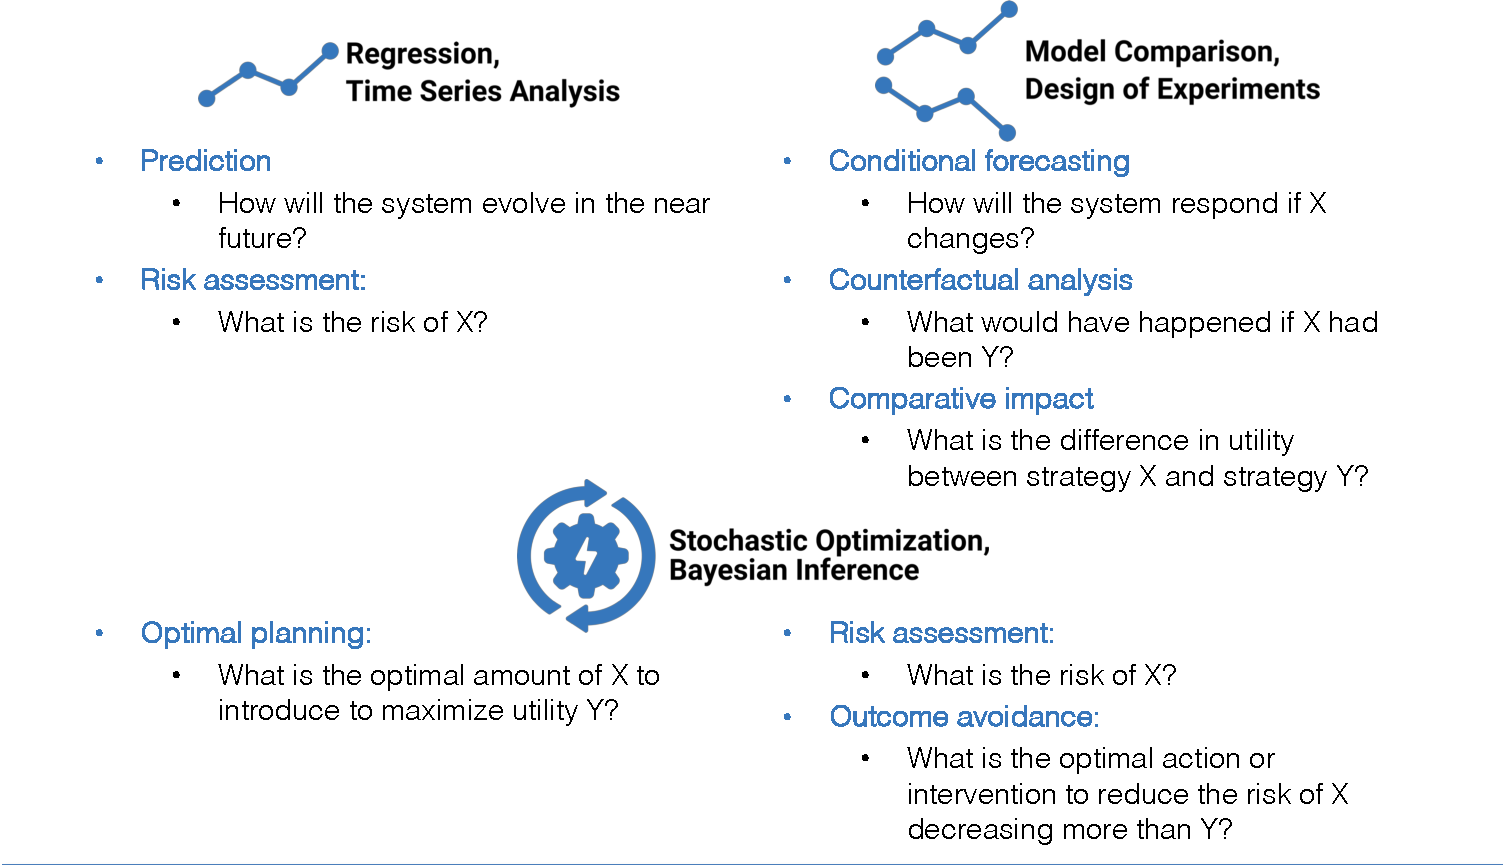
\includegraphics[width=\textwidth]{figs/table.pdf}
  \caption{}
  \label{Fig:InferenceClasses}
\end{figure}

\amidol{} aims to support a number of complex queries and prognostics, as shown in Figure \ref{Fig:InferenceClasses}.  To support a rich interface, we will make use of a Design of Experiments \cite{montgomery2017design} interface coupled with a results database.  Design of Experiments in \amidol{} borrows from concepts of Plackett-Burman designs, and factorial designs using individual reward variables and parameterizations defined over a given model as atomic components of expressions, resulting in new results.  Computations for given atomic components are stored in the results database to avoid unneeded reevaluation, and to allow future experiments to build on past results.

The Design of Experiments interface will allow users to load data from external sources, and associate this data with expectations for state variables in the model.  In our early tests we have achieved this by using data from the CDC's Fluview \cite{cdc2019fluview} data sets as series of instant-of-time observations.  \amidol{}'s interface allows users to use regression to estimate the conditional expectation of dependent variables, given independent variables with fixed values from the data, allowing prediction, parameter estimation, and later risk assessment for a given regression through analysis of the distribution of possible realizations for state variables in a given model.

Models can be compared in our planned Design of Experiments interface by identifying reward variables, or expressions on reward variables, in two models which should be compared and analyzed to explore alternatives, perform conditional forecasting, counterfactual analysis, and comparative impact.  Different strategies, configurations, or possible outcomes can be explored through examining different ways to parameterize a given model, or even differences in models with structural changes.  Debugging experiments will be enabled through the connections to the VDSOL ontology.  For instance, the interface will allow users to see the direct dependence of reward variables to noun's and verbs in the original ontology, better enabling researchers to understand the knowledge-based semantic dependencies normally hidden by traditional modeling techniques.

Sensitivity, uncertainty, and correctness measures can easily be constructed in the planned Design of Experiments interface.  Because we allow for factorial and Plackett-Burman experiment design users can automatically perform one-factor-at-a-time \cite{bailis2005mortality,murphy2004quantification} sensitivity and uncertainty estimates.  The initial prototype will also feature screening sampling-based methods \cite{morris1991factorial} which have been shown to be computationally efficient and are further enabled by our VDSOL ontologies, as they help identify sources of uncertainty and error in the structure of the model.  Correctness is enabled by loading external data from multiple time series or sources, and asking the interface to perform cross validation on the input.  \amidol{} will automatically support k-fold cross validation on time series, allowing automatic partitioning of data sets.

\section{Domain Models}

We are currently testing \amidol{} using several domain models whose primary domain is epidemiology.  We have selected a range of models to test different scenarios, use cases, and assumptions to aid in the prototype design of \amidol{}.

\subsection{SIS/SIRS}

The SIS/SIRS model is one of the simplest models we have deployed for testing with \amidol{}, with the advantage that the model itself is relatively simple, but utilizes real data, and can be used to answer important epidemiological questions.  The primary objective of the SIS/SIRS model is to identify the \emph{basic reproduction number} associated with an infection, also known as $R_0$, or \emph{r nought}.  $R_0$ was first used in 1952 when studying malaria and is a measure of the potential for an infection to spread through a population.  If $R_0 < 1$, then the infection will die out in the long run.  If $R_0 > 1$, then the infection will spread.  The higher the value of $R_0$, the more difficult it is to control an epidemic.

The importance of estimating $R_0$ has been well established for many historical epidemics, including H1N1 \cite{fraser2009pandemic} and Ebola \cite{fisman2014early}.  This model also lends itself to testing \amidol{}'s Design of Experiments module via the plentiful CDC Data \cite{cdc2019fluview} which is well modeled by SIRS.

Given a 100\% effective vaccine, the proportion of the population that needs to be vaccinated is $1 - 1/R_0$, meaning that $R_0$ can be used to plan disease response.  This assumes a homogenous population, and contains many other simplifying assumptions and does not generalize to more complex numbers.  We have several main goals for SIS/SIRS models:

\begin{enumerate}
\item Fitting the models for the data in hindsight to perform goodness of fit estimates.
\item Finding the \emph{retrospective} $R_0$ estimate over the entire epidemic curve.
\item Finding the \emph{real-time} $R_0$ estimate while the epidemic is ongoing.
\end{enumerate}

\paragraph{Data}: For these models we have worked with the WHO/NREVSS (World Health Organization/National Respiratory and Enteric Virus Surveillance System) data sets at the resolution of Department of Human and Health Services designated regions.

\begin{figure}
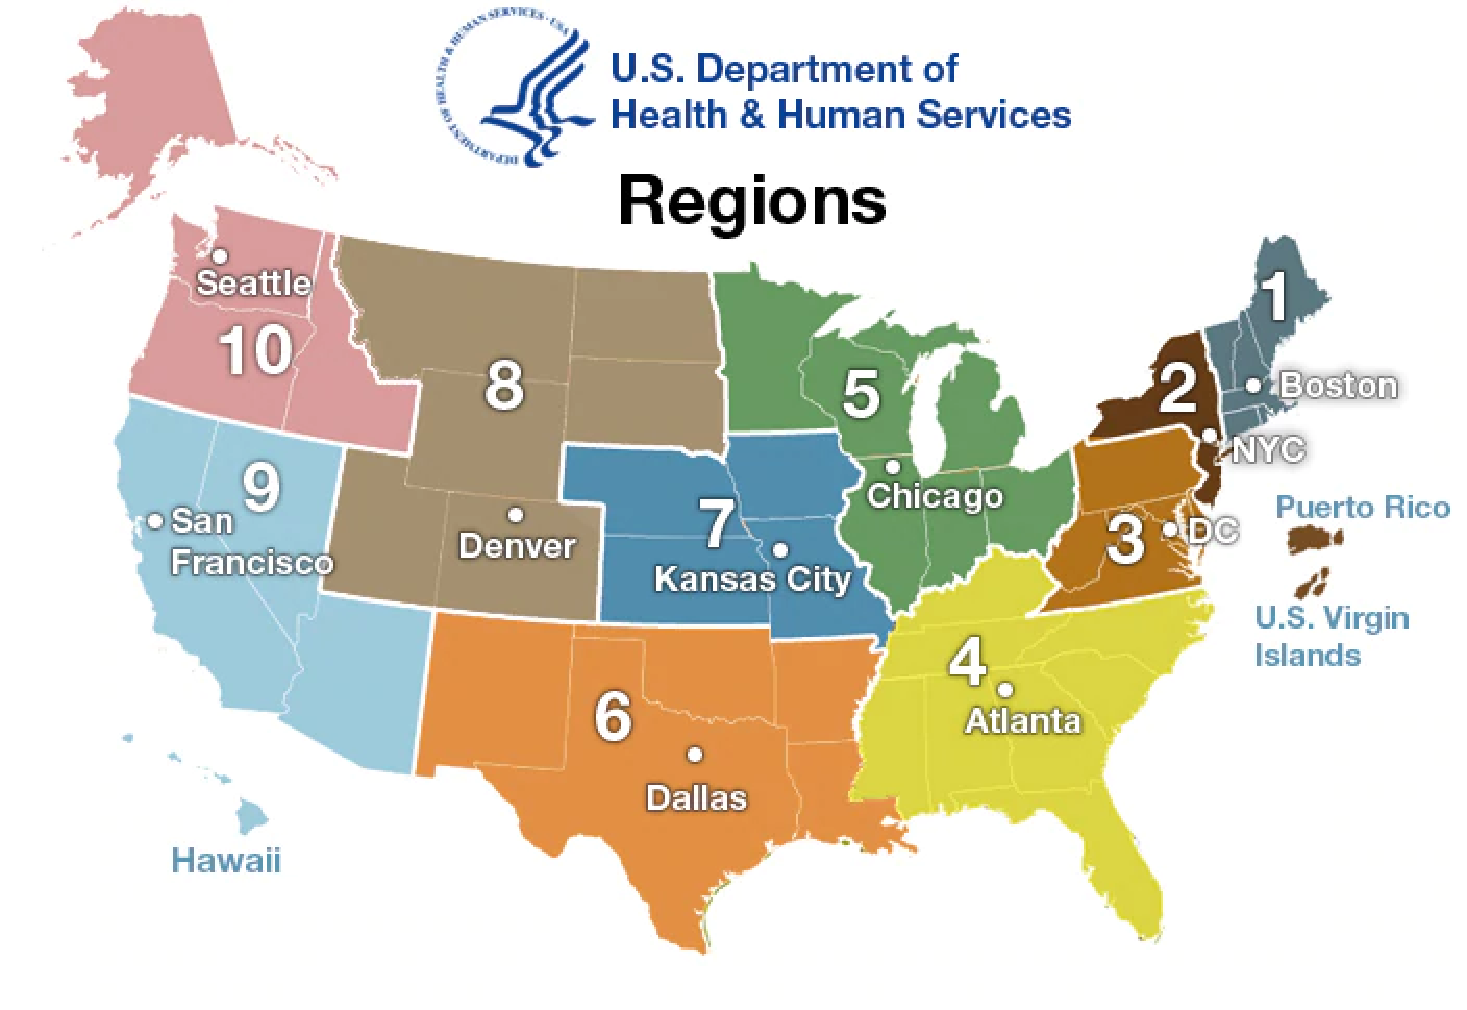
\includegraphics[width=\textwidth]{figs/regionsmap.pdf}
\caption{Department of Human and Health Services designated regions.}
\label{Fig:Regions}
\end{figure}

Using data from a given region, and a given strain, we estimate R0 for the epidemic curve as shown in Figure \ref{Fig:R0}

\begin{figure}
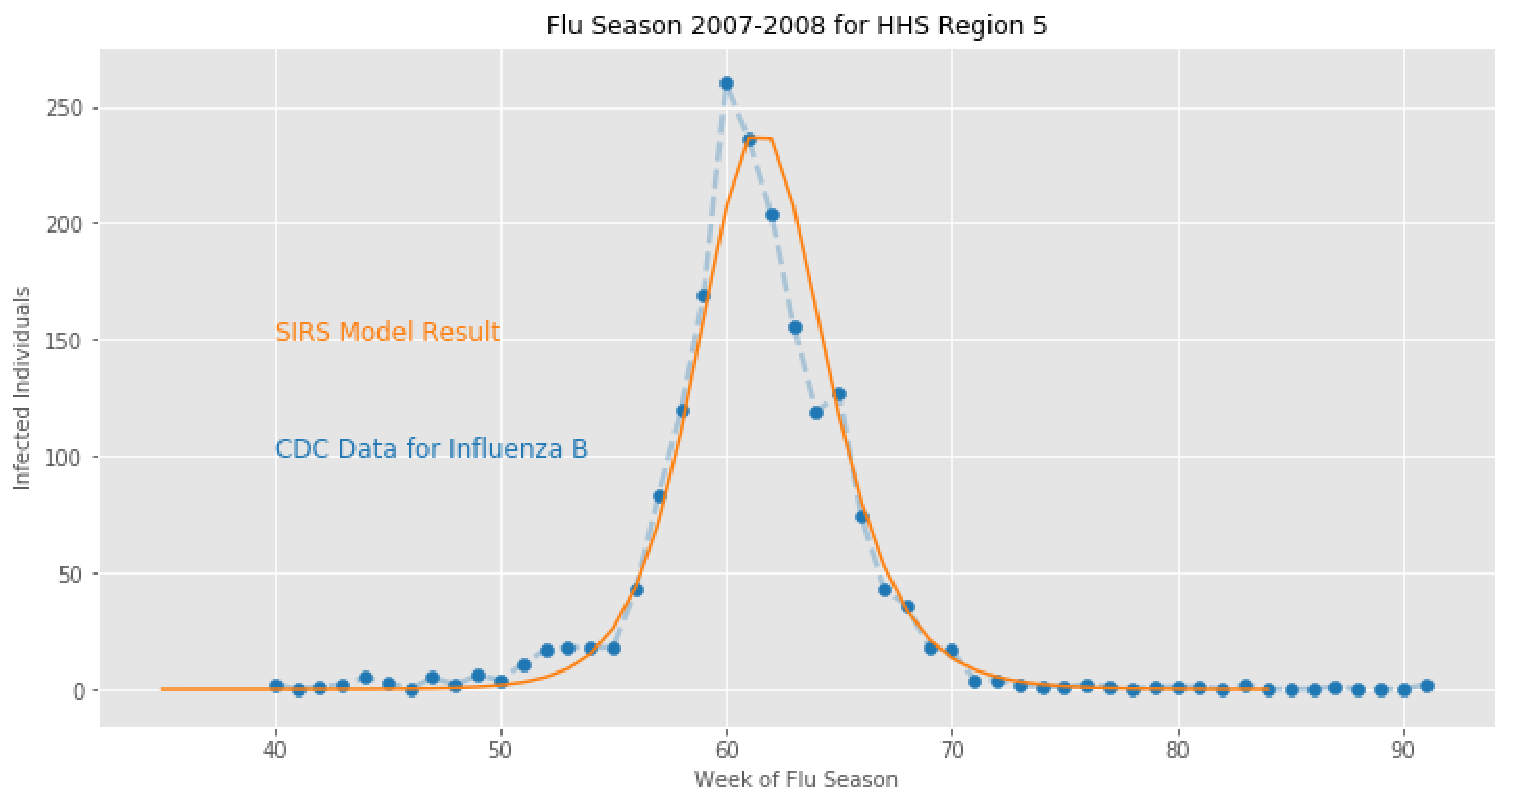
\includegraphics[width=\textwidth]{figs/2007-2008-SIRS.pdf}
\caption{2007 - 2008 Flu Season}
\label{Fig:R0}
\end{figure}

\subsection{Artificial Chemistry and Intracellular Viral Infection}

We have also introduced two simple models of artificial chemistry, and viral infection first introduced by \cite{srivastava2002stochastic,haseltine2002approximate} to test different VDSOLs with similar solution techniques.  While simple, models such as the crystallization model:

\begin{eqnarray}
  2A \overset{e_1}{\rightarrow} B\\
  A + C \overset{e_2}{\rightarrow} D
\end{eqnarray}

Allow us to test features of the UI for \amidol{} in a different domain, and the ability of our predicates to handle non-conservation of value in state variables, along with enabling conditions due to the presence of non-renewable reactions.

\begin{figure}
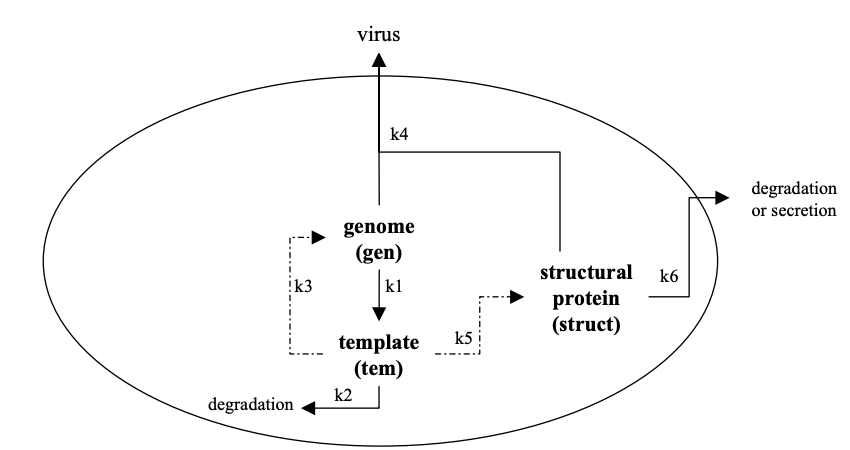
\includegraphics[width=\textwidth]{figs/ViralRep-Crop.png}
\caption{Model of viral replication cycle with catalytic reactions}
\label{Fig:ViralRep}
\end{figure}

Figure \ref{Fig:ViralRep} shows a more complex version of the crystallization model with catalysts, which models viral replication using a chemical kinetic model.

\begin{eqnarray}
\mathrm{nucleotides} \overset{e_1}{\rightarrow} \mathrm{genome}\\
\mathrm{nucleotides} + \mathrm{genome} \overset{e_2}{\rightarrow} \mathrm{template}\\
\mathrm{nucleotides} + \mathrm{aminoacids} \overset{e_3}{\rightarrow} \mathrm{struct}\\
\mathrm{template} \overset{e_4}{\rightarrow} \mathrm{degraded}\\
\mathrm{struct} \overset{e_5}{\rightarrow} \mathrm{secreted}\\
\mathrm{struct} \overset{e_5}{\rightarrow} \mathrm{degraded}\\
\mathrm{genome} + \mathrm{struct} \overset{e_6}{\rightarrow} \mathrm{virus}\\
\end{eqnarray}

This model also features competing events, allowing us to further test our backend's capability for dealing with cases of multiple enabled events.

\subsection{HIV Transactivation Model}

We also employ the HIV Transactivation model presented in \cite{weinberger2005stochastic} as a more complex model of an epidemic process, with the added challenge of handling a system which is stiff, and thus difficult to solve efficiently.  The base model is shown in Figures \ref{Fig:HIV-Tat} and \ref{Fig:HIV-Tat-VDSOL}

\begin{figure}
\begin{subfigure}[b]{\textwidth}
\includegraphics[width=\textwidth]{figs/HIV-Tat-figure.pdf}
\caption{Semi-formal diagram of the molecular model of the Tat transactivation circuit.}
\label{Fig:HIV-Tat}
\end{subfigure}
\begin{subfigure}[b]{\textwidth}
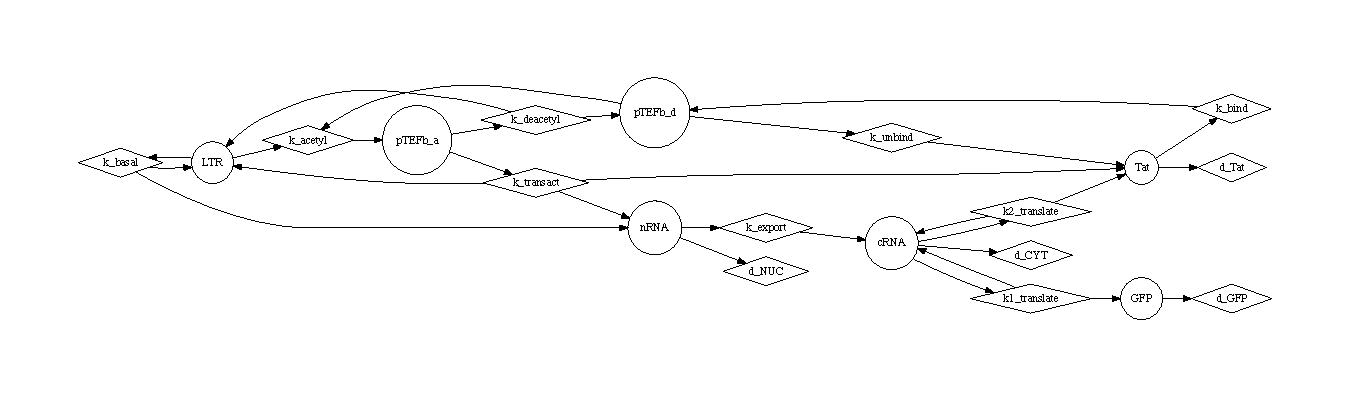
\includegraphics[width=\textwidth]{figs/TatModel.pdf}
\caption{Simple noun (circle) and verb (square) representation of Tat model without ambiguity and aliasing.}
\label{Fig:HIV-Tat-VDSOL}
\end{subfigure}
\end{figure}

Note the use of multiple "Tat" symbols in Figure \ref{Fig:HIV-Tat}. Sometimes scientists draw the same symbol multiple places as an "alias" for the same underlying state variable, which has added the requirement to \amidol{} of supporting entity resolution.  Our goal with \amidol{} is not to fundamentally restrict a domain scientist when drawing diagrams, but rather to assist them in their natural process, and allow them to use the same conventions they are already familiar with, and which exist in their field.

The equations governing this model are given by:

\begin{eqnarray}
LTR \overset{k_{basal}}{\rightarrow} LTR + nRNA\\
nRNA \overset{k_{export}}{\rightarrow} cRNA\\
  cRNA \overset{k1_{translate}}{\rightarrow} GFP + cRNA\\
  cRNA \overset{k2_{translate}}{\rightarrow} Tat + cRNA\\
  Tat \overset{k_{bind}/k_{unbind}}{\leftrightarrow} pTEFb_d\\
  LTR + pTEFb_d \overset{k_{acetyl}/k_{deacetly}}{\leftrightarrow} pTEFb_a\\
  pTEFb_a \overset{k_{transact}}{\leftrightarrow} LTR + nRNA + Tat\\
  GFP \overset{d_{GFP}}{\rightarrow} \emptyset\\
  Tat \overset{d_{Tat}}{\rightarrow} \emptyset\\
  cRNA \overset{d_{CYT}}{\rightarrow} \emptyset\\
  nRNA \overset{d_{NUC}}{\rightarrow} \emptyset
\end{eqnarray}

Using real data generated with flow cytometry, this model can be parameterized as follows:

\begin{eqnarray}
k_basal &=& 10^{-8} (transcripts/s)\\
  k_export &=& 0.00072 (1/s)\\
  k1_translate &=& 0.5 (1/s)\\
  k2_translate &=& 0.005 (1/s)\\
  k_bind &=& 10^{-4} (1/(mol * s))\\
  k_unbind &=& 10^{-2} (1/s)\\
  k_acetyl &=& 10^{-3} (1/(mol * s))\\
  k_deacetyl &=& 0.9 (1/s)\\
  k_transact &=& 0.1 (1/s)
\end{eqnarray}

As can be seen, the rates differ by many orders of magnitude, a situation that causes the model to be classified as stiff, and thus difficult to solve by many ODE techniques.  We are using this model to test the Design of Experiments capability of \amidol{} to automatically select appropriate solution techniques for a user, avoiding numerical instability and the use of inefficient algorithms which otherwise could be pitfalls for traditional modeling methods.

\section{Code Repositories and Current Builds}

The current build of \amidol{} is available in our repository under the \texttt{ir} and \texttt{ui} directories.  Both of which have instructions on building and executing the current system.  Models can be designed in the current VDSOL editor, an Elm project contained in the `ui` directory, which is implemented as a series of
web applications produced by the Elm compiler as HTML, CSS, and Javascript. Current capabilities include drawing/manipulating semi-formal models, issuing queries, and loading data.

The intermediate representation is implemented as a Scala project contained in the `ir` directory.  It compiles queries issued by users for a particular model they've created into code artifacts targeting different solver backends. Over time, we expect this
system to also manipulate and compose datasets (from real-world observations
as well as from the output of other simulations), and utilize the results database.


\subsection{Front-End Architecture for VDSOLs}

\begin{figure}
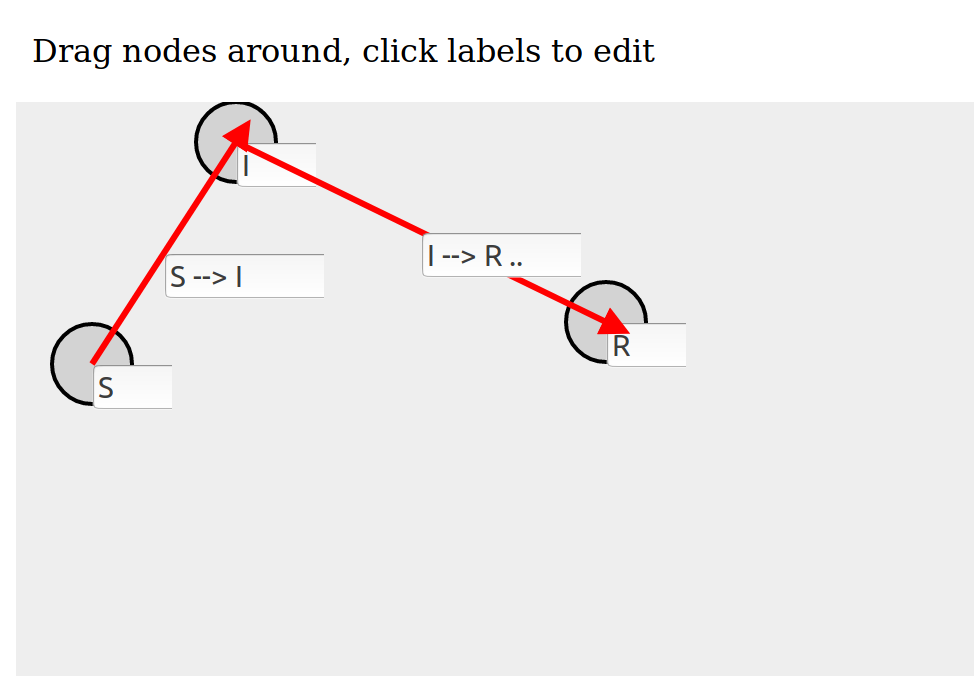
\includegraphics[width=\textwidth]{figs/Editor.png}
\caption{Current Front-End featuring a generic VDSOL.  The front-end enables the embedding of custom SVGs for nouns and verbs, allowing eventual specialization of produced figures, better matching current domain conventions.}
\label{Fig:Editor}
\end{figure}

\amidol{}'s user interface is a small collection of web pages which communicate with the Scala back-end using JSON over HTTP.  This client/server approach leverages standard browser technologies like HTML5, CSS, and SVG graphics for rapid development of rich interactions tailored for the specific needs of scientific modeling. It also decouples the concerns of visual presentation and manipulation from the underlying representations of model semantics.

The Javascript code which implements the user interface is compiled from Elm, a strongly typed functional language designed specifically for front-end web development. Elm's runtime system is similar to that of popular Javascript frameworks like React, but the language provides some distinct advantages in terms of correctness, performance, and ease of refactoring. In addition to the capabilities provided by the Elm package ecosystem, Elm applications can interoperate directly with Javascript, allowing \amidol to make use of the best available web-based data visualization libraries.

Integration concepts:
\begin{itemize}
\item API schema and versioning
\item supports collaboration between multiple users
\item one server, potentially multiple client implementations
\item persistent server, ephemeral clients
\item resource-heavy clusters, lightweight clients
\end{itemize}

Currently, the user interface implements a visual editor for directed graphs having labeled vertices and edges, which represent the nouns and verbs of a VDSOL. We are in the process of designing a set of user interactions with these graph models, including save / load, model composition, and various forms of simulation analysis and query generation. The UI will also show the responses to users' queries in appropriate visual forms, such as multivariate time-series plots.

\subsection{Backend Architecture for IR and Inference Engine}

\begin{figure}
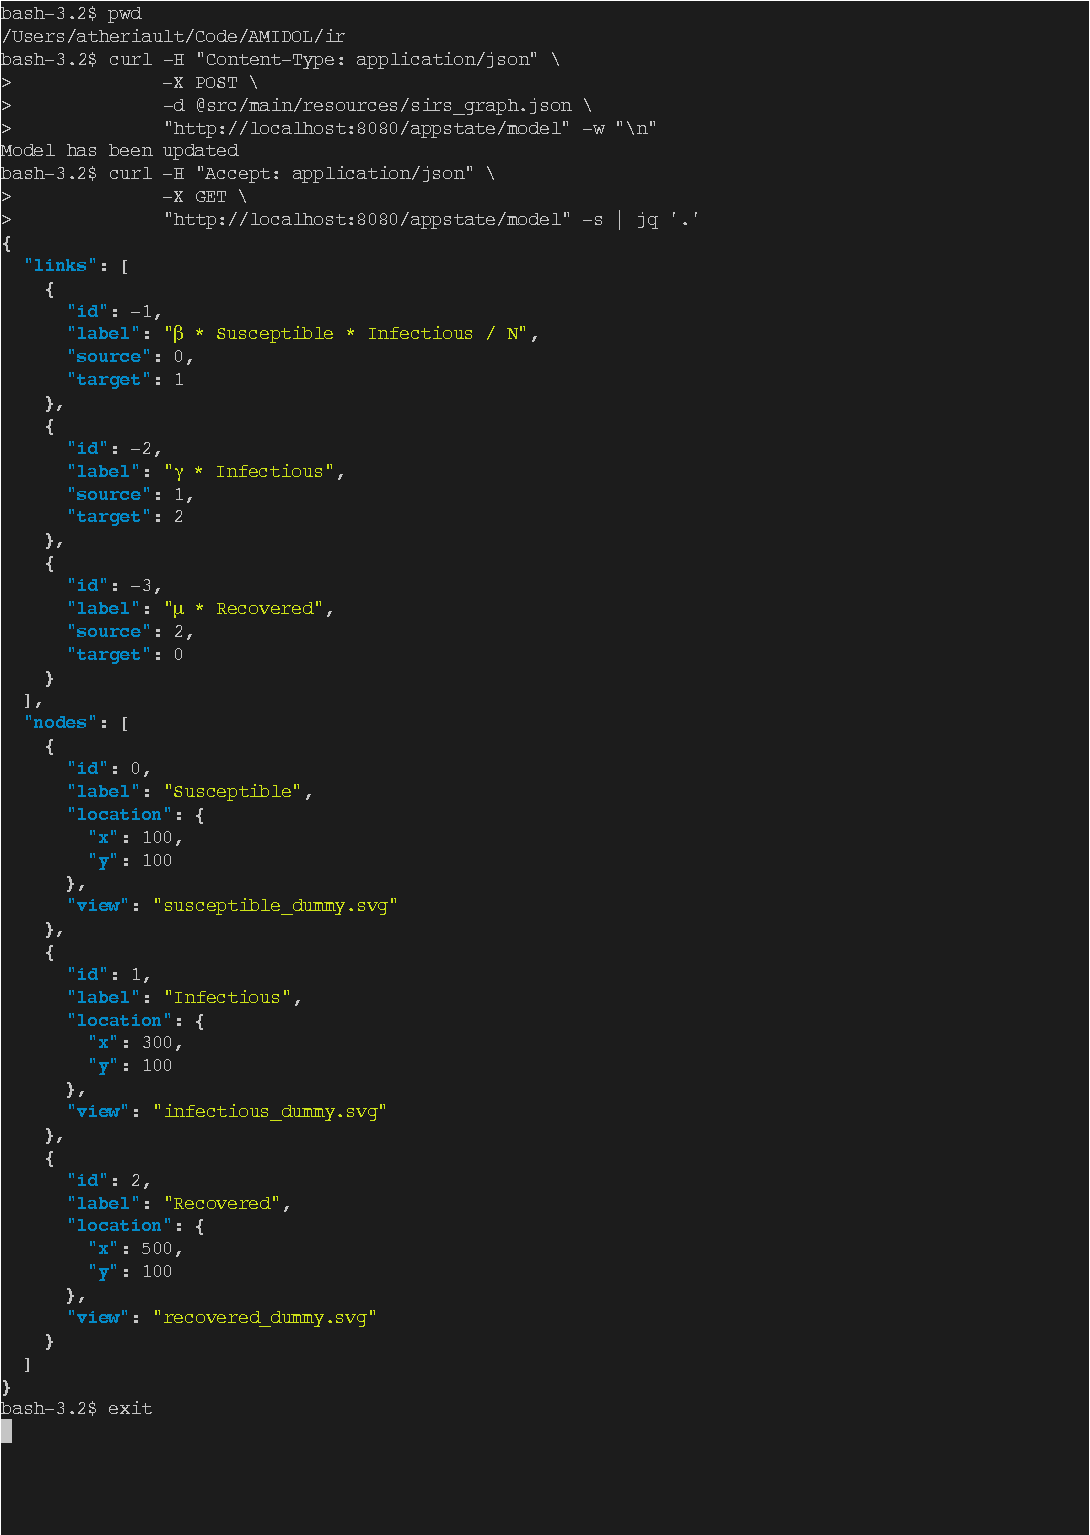
\includegraphics[width=\textwidth]{figs/LoadModel-crop.pdf}
\caption{Example of the AFI/IR loading a model produced in the VDSOL, and parsing it into the intermediate representation.}
\label{Fig:LoadModel}
\end{figure}

\begin{figure}
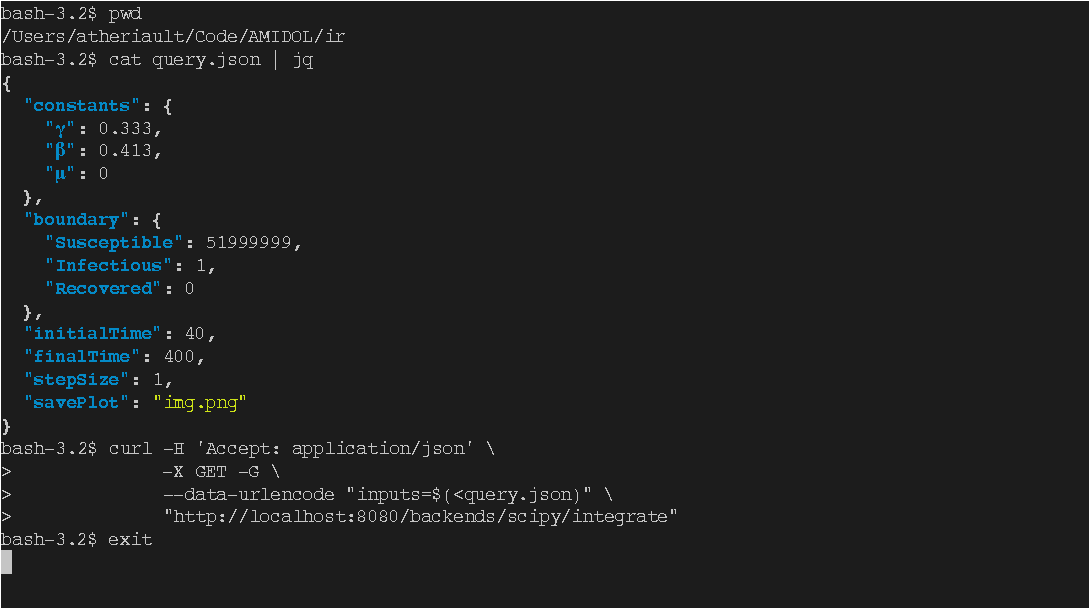
\includegraphics[width=\textwidth]{figs/QueryIntegrateBackend-crop.pdf}
\caption{Example of the AFI/IR running a query on a translated model using SciPy as the backend target to produce time series estimates.}
\label{Fig:Query}
\end{figure}

The backend component interfaces with the UI via a local web server. The idea here is that every time the user interacts with the UI either to modify or to query the model, that information also gets relayed to the backend via a set of web endpoints. When the backend receives new information about the model from the UI, it parses this into some internal representation. This includes such tasks as parsing equations from user-inputted strings and checking that state variables being referred to actually exist. Queries submitted about a model follow a slightly longer path: after being parsed out and validated, the backend figures out how to transform the IR and the query into executable code using reward variables, executes this code, and returns the result back out to the user and eventual results database.

Within the backend, the IR is stored in a graph format resembling what the user constructed in the UI. By maintaining some degree of similarity, we hope to make it simpler to translate results obtained in the backend back out into something end users can easily understand. Queries about models are translated into code artifacts targeting existing solver and simulation programs. We wish to avoid doing actual simulations within the system, instead focusing on intelligently compiling queries into programs that external solvers can run allowing code reuse, and allowing the backend to generate targets for existing, high performance, solver engines. In order to do this we still need to implement a minimum amount of symbolic algebra (e.g. detecting when a continuous rate  model is linear). For the time being, we’ve been targeting Python’s SciPy module as a backend to answer basic simulation questions such as: the the initial value problem for general systems as well as for continuous-time Markov chains.

The backend is written in Scala, leveraging a set of libraries built on top of the Akka actor system for the web server, JSON processing, asynchronous computation, and eventually for the graph in which the IR and data will be stored. The advantages to using Scala include: deployable anywhere the JVM runs, large set of available libraries, and a functional outlook which lends itself well to compiler problems.

\subsection{Integrating AMIDOL}

\begin{figure}
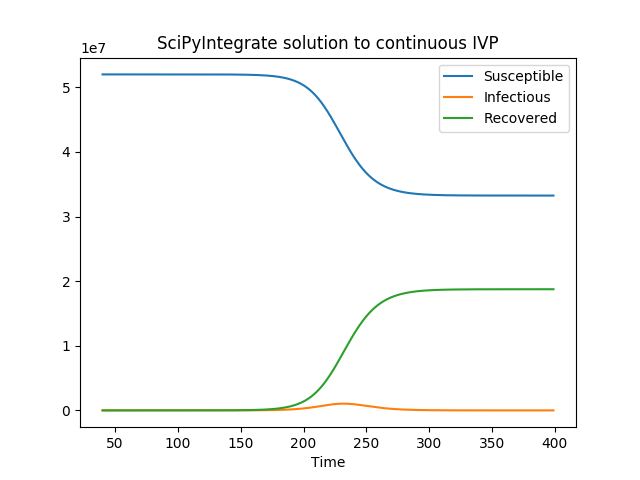
\includegraphics[width=\textwidth]{figs/QueryResult.png}
\caption{Query Results returned from the AFI/IR backend to the VDSOL frontend displaying values over a defined set of instant-of-time rate reward variables.}
\label{Fig:QueryResult}
\end{figure}

The JSON API which defines client/server interaction is the only channel by which tangible VDSOL models and the computational AFI/IR communicate. The UI itself doesn't hold any persistent model state which is not represented in a given VDSOL; it is precisely a view or translation of the AFI/IR. This property is what enables the list of integration concepts, and restful architecture.

\bibliography{AMIDOL-MWS}



\end{document}

%  LocalWords:  textbf Composability lampka2002symbolic mathbb ldots
%  LocalWords:  sanders1992dependability,sanders1988construction cdot
%  LocalWords:  sanders1995ultrasan rightarrow infty mathcal cdot t,t
%  LocalWords:  qureshi1996algorithms,deavours1999efficient,ciardo1996well
%  LocalWords:  freire1990technique t,t includegraphics textwidth
%  LocalWords:  Plackett-Burman Fluview cdc2019fluview eqnarray
%  LocalWords:  bailis2005mortality,murphy2004quantification mathrm
%  LocalWords:  morris1991factorial fraser2009pandemic mathrm texttt
%  LocalWords:  fisman2014early aminoacids weinberger2005stochastic
%  LocalWords:  srivastava2002stochastic,haseltine2002approximate
%  LocalWords:  deacetly emptyset cytometry k_deacetyl texttt
